
% This LaTeX was auto-generated from an M-file by MATLAB.
% To make changes, update the M-file and republish this document.

\documentclass{article}
\usepackage{graphicx}
\usepackage{color}
\usepackage{listings}
\usepackage[framed]{mcode}
\usepackage{fullpage}
\usepackage{amsmath}
\usepackage[utf8x]{inputenc}
\usepackage{import}
\usepackage{setspace}
\usepackage{hyperref}
\definecolor{lightgray}{gray}{0.5}
\setlength{\parindent}{0pt}

\begin{document}

    
    
%\section*{}


\title{BE 521: Homework 6 \\{\normalsize Spike sorting}\\{\normalsize Spring 2021}}
\author{60 points}
\date{Due: Tuesday, 03/09/2021 10:00pm}
\maketitle \textbf{Objective:} Detect and cluster spikes


\begin{center} \author{NAME HERE \\
  \normalsize Collaborators: COLLABORATORS HERE \\}
\end{center}


\subsection*{Overview}
In this homework, you will do some basic spike sorting using two different datasets. The first (\verb|I521_A0006_D001|) is from a crayfish neuromuscular junction, a good model for human central nervous system synapses\footnote{The sampling rate of this data is 2000 Hz, which is adequate for this homework's instructional purposes but usually inadequate for real spike sorting, which often uses sampling frequencies on the order of 20 kHz.}. Specifically, the data contains two simultaneous recordings: an extracellular recording from the third nerve (channel \verb|nerve|) of a crayfish abdominal ganglion, which contains six spontaneously active motor neurons, and an intracellular recording from the superficial flexor muscle (channel \verb|muscle|) innervated by this nerve. You will attempt to discern relationships between the classes of spike waveforms you extract from the motor nerve trace and elicited potentials seen in the muscle fiber recording.
Then, you will revisit a human intracranial EEG recording (\verb|I521_A0006_D002|) and use some of the techniques you've learned in class to build a more automated spike sorter.
Note: While spikes may have positive and negative deflections, we will only focus on positive spikes on this homework for simplicity.
\section{Spike Detection and Clustering (38 pts)}
In this section, you will explore some basic filtering and spike thresholding to ultimately compare spike clusters you pick out by eye to those selected by an automated algorithm.
\begin{enumerate}
    \item You can assume that the nerve samples have already been low-pass filtered. Here you will high-pass filter in order to remove signals like slow local field potentials and 60 Hz power line noise. Create a 4th order \textit{elliptic filter} with 0.1 dB of ripple in the passband, a stopband 40 dB lower than the peak value in the passband, and a passband edge frequency of 300 Hz (see Matlab's \verb|ellip| function and make sure your give the edge frequency in the correct normalized form). The statement to create this filter (defined by the filter coefficients \verb|b| and \verb|a|) should look something like
  \begin{lstlisting}
	[b,a]=ellip(n,Rp,Rs,Wp,'high')
  \end{lstlisting}
  Clearly specify the denominator and numerator coefficients obtained for your filter function. (2pts)

\begin{lstlisting}
cd('/Users/sppatankar/Developer/BE-521')
addpath(genpath('Homework_6'));
addpath(genpath('ieeg-matlab-1.14.49'))

session_1 = IEEGSession('I521_A0006_D001', 'spatank', 'spa_ieeglogin.bin');

sampling_rate_1 = session_1.data.sampleRate;
n = 4; % fourth-order filter
Rp = 0.1; % ripple in the passband
Rs = 40; % attenuation in the stopband
Wp = 300/(sampling_rate_1/2); % normalized passband edge frequency
[b, a] = ellip(n, Rp, Rs, Wp, 'high')
\end{lstlisting}

\color{lightgray} \begin{lstlisting}IEEGSETUP: Adding 'ieeg-matlab.jar' to dynamic classpath
Warning: Objects of edu/upenn/cis/db/mefview/services/TimeSeriesDetails class
exist - not clearing java 
Warning: Objects of edu/upenn/cis/db/mefview/services/TimeSeriesInterface class
exist - not clearing java 
IEEGSETUP: Found log4j on Java classpath.
URL: https://www.ieeg.org/services
Client user: spatank
Client password: ****

b =

    0.3420   -1.2740    1.8676   -1.2740    0.3420


a =

    1.0000   -1.7432    1.6167   -0.6559    0.1430

\end{lstlisting} \color{black}

  \item Using the \verb|filter| function and \verb|filtfilt| function, obtain two different filtered outputs of the nerve signal.
      \begin{enumerate}
        \item In a 2x1 subplot, plot the first 50 ms of the unfiltered nerve signal in the top subplot; in the bottom subplot, plot the \verb|filter| output in blue and the \verb|filtfilt| output in red. Use a potential range (y-axis) of -20 to 50 millivolts. (4 pts)

\begin{lstlisting}
end_time_nerve = session_1.data.rawChannels(2).get_tsdetails.getEndTime/1e6; % s
time_nerve = 0:1/sampling_rate_1:end_time_nerve;
nerve_signal = session_1.data.getvalues(1:ceil(end_time_nerve * sampling_rate_1), 2); % microV
nerve_signal_filtfilt = filtfilt(b, a, nerve_signal);
nerve_signal_filter = filter(b, a, nerve_signal);

figure;
subplot(2, 1, 1);
plot(time_nerve(1:round(sampling_rate_1 * 50 / 1000)) * 10^3, ...
    nerve_signal(1:round(sampling_rate_1 * 50 / 1000)) / 10^3, ...
    'LineWidth', 2, 'Color', [0, 0, 0])
% ylim([-20, 50])
xlabel('Time (ms)', 'FontSize', 15);
ylabel('Nerve Signal (mV)', 'FontSize', 15);
subplot(2, 1, 2);
hold on
plot(time_nerve(1:round(sampling_rate_1 * 50 / 1000)) * 10^3, ...
    nerve_signal_filter(1:round(sampling_rate_1 * 50 / 1000)) / 10^3, ...
    'LineWidth', 2, 'Color', 'b')
plot(time_nerve(1:round(sampling_rate_1 * 50 / 1000)) * 10^3, ...
    nerve_signal_filtfilt(1:round(sampling_rate_1 * 50 / 1000)) / 10^3, ...
    'LineWidth', 2, 'Color', 'r')
legend('filter()', 'filtfilt()', 'Location', 'Best');
% ylim([-20, 50])
hold off
xlabel('Time (ms)', 'FontSize', 15);
ylabel('Nerve Signal (mV)', 'FontSize', 15);
\end{lstlisting}


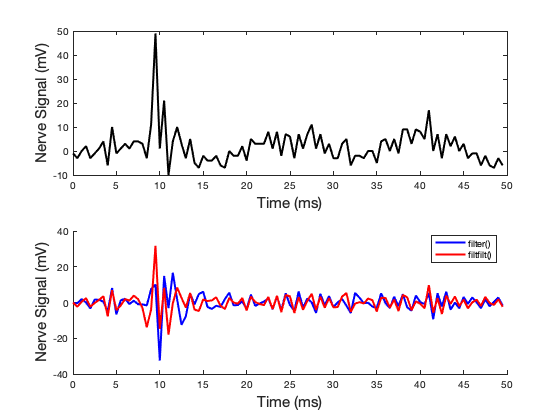
\includegraphics [width=5in]{spatank_hw6_01.png}

        \item How is the unfiltered signal different from the filtered signal? What is different about the two filtered (red and blue) signals? (2 pts)


        \item Briefly explain the mathematical difference between the two filtering methods, and why one method might be more advantageous than the other in the context of spike detection? (5 pts)


      \end{enumerate}
        \item Using a spike threshold of +30 mV, calculate the index and value of the peak voltage for each spike in the \textbf{filtered} nerve signal (select the best one). Use these values to plot the first 2.5 seconds of the nerve signal with a red dot above (e.g. 10 mV above) each spike. (Hint: Plot the entire length of the nerve signal with all the spikes marked but then restrict the x-axis using \verb|xlim| to [0, 2.5] seconds) (4 pts)

\begin{lstlisting}
threshold = 30 * 10^3; % microV
inds_df_2 = diff(diff(nerve_signal_filtfilt) < 0);
inds_thresh = nerve_signal_filtfilt(2:end-1) > threshold;
inds = find(inds_df_2 .* inds_thresh);
vals = nerve_signal_filtfilt(inds + 1);

figure;
hold on
plot(time_nerve, nerve_signal_filtfilt / 10^3, 'Color', [0, 0, 0]);
plot(inds/sampling_rate_1, (vals / 10^3) + 10, 'r.', 'MarkerSize', 10);
hold off
xlim([0, 2.5])
xlabel('Time (s)', 'FontSize', 15);
ylabel('mV', 'FontSize', 15);
title('Nerve Signal with Spikes', 'FontSize', 15);
\end{lstlisting}


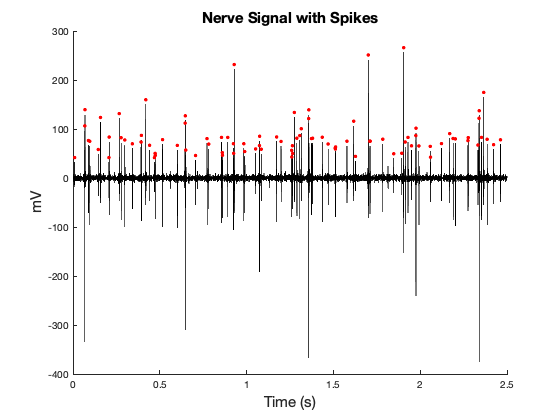
\includegraphics [width=5in]{spatank_hw6_02.png}

 \item Under the assumption that different cells produce different action potentials with distinct peak amplitudes, decide how many cells you think were recorded (some number between 1 and 6). You may find it helpful to zoom in and pan on the plot you made in question 1.3. You may also find it useful to plot the sorted peak values to gain insight into where ``plateaus'' might be. (No need to include these preliminary plots in the report, though.) Use thresholds (which you well set manually/by eye) to separate the different spikes. Make a plot of the first 2.5 seconds similar to that in 1.3 except now color the spike dots of each group a different color (e.g., \verb|'r.'|,\verb|'g.'|,\verb|'k.'|,\verb|'m.'|).(6 pts)

\begin{lstlisting}
% [sorted_vals, sorted_idx] = sort(vals);
% figure;
% plot((sorted_vals / 10^3), 'r.', 'MarkerSize', 10);
% ylabel('mV', 'FontSize', 15);

thresholds = [60, 85, 170, 260];

figure; cla;
plot(time_nerve, nerve_signal_filtfilt / 10^3, 'Color', [0, 0, 0]);
hold on
for i = 1:length(vals)
    val = vals(i) / 10^3;
    if val > 0 && val <= 60
        style = 'r.';
    end
    if val > 60 && val <= 85
        style = 'g.';
    end
    if val > 85 && val <= 170
        style = 'k.';
    end
    if val > 170 && val <= 260
        style = 'm.';
    end
    plot(inds(i)/sampling_rate_1, (vals(i) / 10^3) + 10, style, ...
        'MarkerSize', 10);
end
hold off
xlim([0, 2.5])
xlabel('Time (s)', 'FontSize', 15);
ylabel('mV', 'FontSize', 15);
title('Manually Sorted Spikes', 'FontSize', 15);
\end{lstlisting}


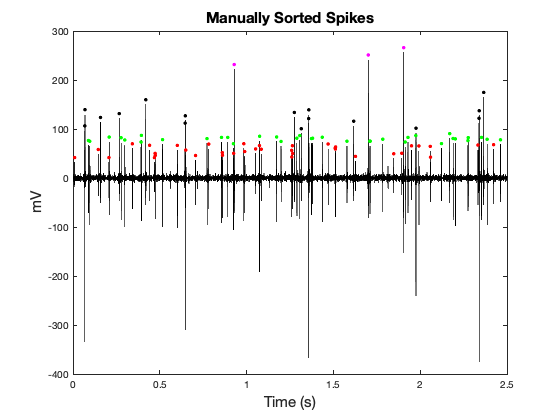
\includegraphics [width=5in]{spatank_hw6_03.png}

 \item Use Matlab's $k$-means\footnote{Clustering, like $k$-means you are using here, is a form of unsupervised learning.} function (\verb|kmeans|) to fit $k$ clusters (where $k$ is the number of cells you think the recording is picking up) to the 1D data for each spike.
  \begin{enumerate}
	\item Using the same color order (for increasing spike amplitude) as you did for the thresholds in question 1.4, plot the spike cluster colors as little dots slightly above those you made for question 1.4. The final figure should be a new plot of the nerve voltage and two dots above each spike, the first being your manual label and the second your clustered label, which (hopefully/usually) should be the same color. (4 pts)

\begin{lstlisting}
[labels, C] = kmeans(vals, 4);
C = C/10^3;

styles = {'r.', 'g.', 'k.', 'm.'};
[centroids, sort_idx] = sort(C);

figure; cla;
plot(time_nerve, nerve_signal_filtfilt / 10^3, 'Color', [0, 0, 0]);
hold on
for i = 1:length(vals)
    % manual clustering
    val = vals(i) / 10^3;
    if val > 0 && val <= 60
        style = styles{1};
    end
    if val > 60 && val <= 85
        style = styles{2};
    end
    if val > 85 && val <= 170
        style = styles{3};
    end
    if val > 170 && val <= 260
        style = styles{4};
    end
    plot(inds(i)/sampling_rate_1, (vals(i) / 10^3) + 10, style, ...
        'MarkerSize', 10);
    % kmeans clustering
    if labels(i) == sort_idx(1)
        style_k = styles{1};
    end
    if labels(i) == sort_idx(2)
        style_k = styles{2};
    end
    if labels(i) == sort_idx(3)
        style_k = styles{3};
    end
    if labels(i) == sort_idx(4)
        style_k = styles{4};
    end
    plot(inds(i)/sampling_rate_1, (vals(i) / 10^3) + 20, style_k, ...
        'MarkerSize', 10);
end
hold off
xlim([0, 2.5])
xlabel('Time (s)', 'FontSize', 15);
ylabel('mV', 'FontSize', 15);
title('Manually and k-means Sorted Spikes', 'FontSize', 15);
\end{lstlisting}


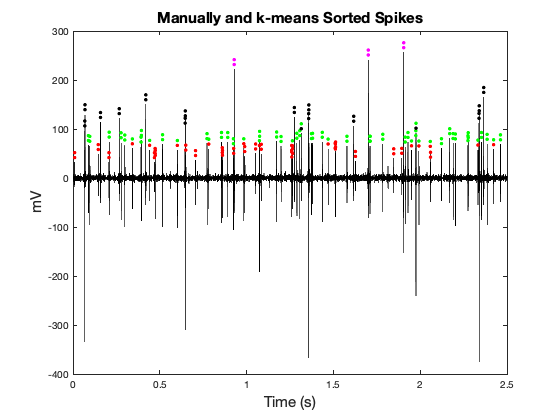
\includegraphics [width=5in]{spatank_hw6_04.png}

	\item Which labeling, your manual ones or the ones learned by clustering) seem best, or do they both seem just as good? (Again, panning over the entire plot may be helpful.) (2 pts)


  \end{enumerate}
 \item In this question,  you will test the hypothesis that the muscle potential responses are really only due to spikes from a subset of the cells you have identified in the previous two questions. First, plot the first 2.5 seconds of the muscle fiber potential and compare it with that of the nerve. Observe the relationship between spikes and the muscle fiber response. (No need to include this plot and observation in your report.)
     Now, calculate the maximum muscle fiber potential change\footnote{max voltage - min voltage} in the 25 ms\footnote{Note that this 25 ms window is somewhat ad hoc and is just what seems reasonable by eye for this data. It implies no underlying physiological time scale or standard.} window after each spike (with the assumption that spikes without any/much effect on the muscle fiber potential do not directly innervate it).
  \begin{enumerate}
   \item Using the cell groups you either manually defined or found via $k$-means clustering (just specify which you're using) again with different colors, plot a colored point for each spike where the x-value is the spike amplitude and the y-value is the muscle potential change. (6 pts)

\begin{lstlisting}
end_time_muscle = session_1.data.rawChannels(1).get_tsdetails.getEndTime/1e6; % s
time_muscle = 0:1/sampling_rate_1:end_time_nerve;
muscle_signal = session_1.data.getvalues(1:ceil(end_time_muscle * sampling_rate_1), 1); % microV

figure;
subplot(2, 1, 1);
plot(time_nerve * 10^3, ...
    nerve_signal / 10^3, ...
    'LineWidth', 2, 'Color', [0, 0, 0])
xlabel('Time (ms)', 'FontSize', 15);
ylabel('Nerve Signal (mV)', 'FontSize', 15);
subplot(2, 1, 2);
plot(time_muscle * 10^3, ...
    muscle_signal / 10^3, ...
    'LineWidth', 2, 'Color', [0, 0, 0])
xlim([0, 2.5 * 10^3])
xlabel('Time (ms)', 'FontSize', 15);
ylabel('Muscle Signal (mV)', 'FontSize', 15);

potential_change = zeros(1, length(vals));

window_size = round(25/1000 * sampling_rate_1);
for i = 1:length(vals)
    spike_idx = inds(i);
    spike_window = muscle_signal(spike_idx:(spike_idx + window_size - 1));
    potential_change(i) = max(spike_window) - min(spike_window);
end

figure; cla;
hold on
for i = 1:length(vals)
    % kmeans clustering
    if labels(i) == sort_idx(1)
        style_k = styles{1};
    end
    if labels(i) == sort_idx(2)
        style_k = styles{2};
    end
    if labels(i) == sort_idx(3)
        style_k = styles{3};
    end
    if labels(i) == sort_idx(4)
        style_k = styles{4};
    end
    plot(vals(i) / 10^3, (potential_change(i) / 10^3), style_k, ...
        'MarkerSize', 10);
end
hold off
xlabel('Spike Amplitude (mV)', 'FontSize', 15);
ylabel('Potential Change (mV)', 'FontSize', 15);
\end{lstlisting}


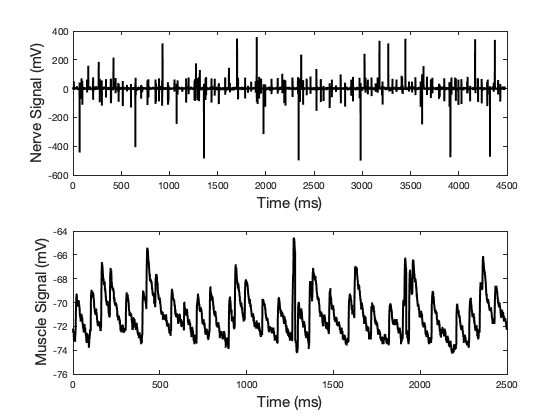
\includegraphics [width=5in]{spatank_hw6_05.png}


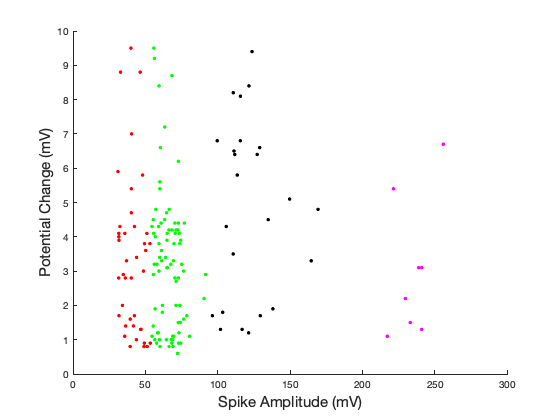
\includegraphics [width=5in]{spatank_hw6_06.png}

   \item Does this plot support the hypothesis that the muscle fiber responses are only due to a subset of the cells. Explain why or why not. (3 pts)


  \end{enumerate}
\end{enumerate}
\section{Multivariate Clustering (22 pts)}
In this section, you will explore similar methods for spikes sorting and clustering but with a different dataset, the human intracranial data in \verb|I521_A0006_D002|,
which is a larger dataset of the same recording you saw in \verb|I521_A0001_D001| of Homework 1.
  \begin{enumerate}
   \item Using a threshold six standard deviations above the mean of the signal, detect the spikes in the signal. In addition, extract the waveform from 1 ms before the peak to 1 ms after it with peak value in the middle. (You will end up with a matrix where each row corresponds to the number of data points in 2 ms of signal minus 1 data point. Use the closest integer number of data points for the $\pm$ 1 ms window.)

\begin{lstlisting}
session_2 = IEEGSession('I521_A0006_D002', 'spatank', 'spa_ieeglogin.bin');
sampling_rate_2 = session_2.data.sampleRate;
end_time = session_2.data.rawChannels(1).get_tsdetails.getEndTime/1e6; % s
time = 0:1/sampling_rate_2:end_time;
signal = session_2.data.getvalues(1:ceil(end_time * sampling_rate_2), 1); % microV

threshold = mean(signal) + (6 * std(signal));
inds_df_2 = diff(diff(signal) < 0);
inds_thresh = signal(2:end-1) > threshold;
inds = find(inds_df_2 .* inds_thresh);
vals = signal(inds + 1);

half_window_size = round((1/1000) * sampling_rate_2) - 1;

all_waveforms = zeros(length(vals), (2 * half_window_size) + 1);
pseudo_time = linspace(-1, 1, (2 * half_window_size) + 1);
\end{lstlisting}

\color{lightgray} \begin{lstlisting}IEEGSETUP: Adding 'ieeg-matlab.jar' to dynamic classpath
Warning: Objects of edu/upenn/cis/db/mefview/services/TimeSeriesDetails class
exist - not clearing java 
Warning: Objects of edu/upenn/cis/db/mefview/services/TimeSeriesInterface class
exist - not clearing java 
IEEGSETUP: Found log4j on Java classpath.
URL: https://www.ieeg.org/services
Client user: spatank
Client password: ****
\end{lstlisting} \color{black}

	\begin{enumerate}
	  \item Plot the waveforms of all the spikes overlaid on each other in the same color. (4 pts)

\begin{lstlisting}
figure; cla;
hold on
for i = 1:length(vals)
    curr_spike_start = inds(i);
    all_waveforms(i, :) = ...
        signal(inds(i) - half_window_size:inds(i) + half_window_size);
    plot(pseudo_time, all_waveforms(i, :), 'LineWidth', 0.25, 'Color', 'k', ...
        'MarkerSize', 10);
end
hold off
xlabel('Time from Spike (ms)', 'FontSize', 15);
ylabel('Signal ({\mu}V)', 'FontSize', 15);
title('Spike Waveform', 'FontSize', 15);
\end{lstlisting}


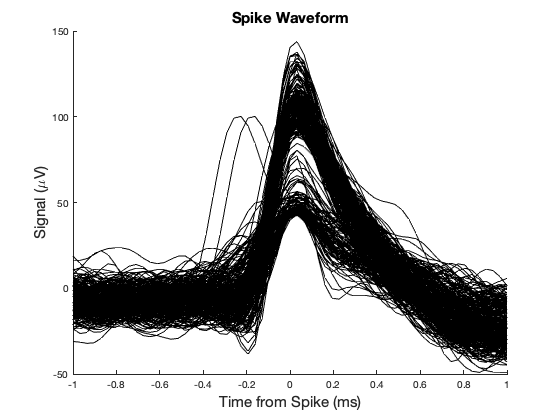
\includegraphics [width=5in]{spatank_hw6_07.png}

	  \item Does it looks like there is more than one type of spike? (1 pt)


	\end{enumerate}
   \item For each spike, represent the waveform by its  principal components. Use the \verb|pca| command in Matlab. Intuitively, principal component analysis finds the coordinate system that most reduces the variability in your data.
	\begin{enumerate}
	  \item Run principal component analysis on all the spike waveforms and represent your data with the top two principal components. Make a scatterplot of your data in this principal component (PC) space. (3 pts)

\begin{lstlisting}
[coeff, score, latent, tsquared, explained] = pca(all_waveforms);

figure;
plot(score(:, 1), score(:, 2), 'k.', 'MarkerSize', 10)
xlabel('1st Principal Component', 'FontSize', 15)
ylabel('2nd Principal Component', 'FontSize', 15)
title('Spike Waveform PCs', 'FontSize', 15);
\end{lstlisting}


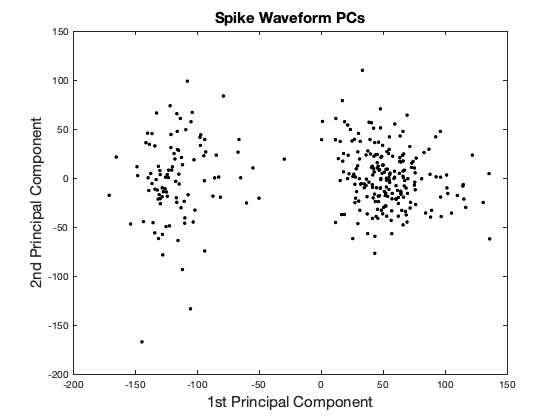
\includegraphics [width=5in]{spatank_hw6_08.png}

	  \item Each PC also has an associated eigenvalue, representing the amount of variance explained by that PC. This an output of the \verb|PCA| command. Plot the  principal component vs the total (cumulative) percent variance explained. What is the percent variance explained if you include the top two principal components? (3 pts)

\begin{lstlisting}
figure;
plot(1:size(score, 2), cumsum(explained), 'LineWidth', 2, 'Color', [0, 0, 0])
xlabel('Number of PCs', 'FontSize', 15)
ylabel('Percentage of Variance Explained', 'FontSize', 15)
title('Spike Waveform PCs', 'FontSize', 15);
\end{lstlisting}


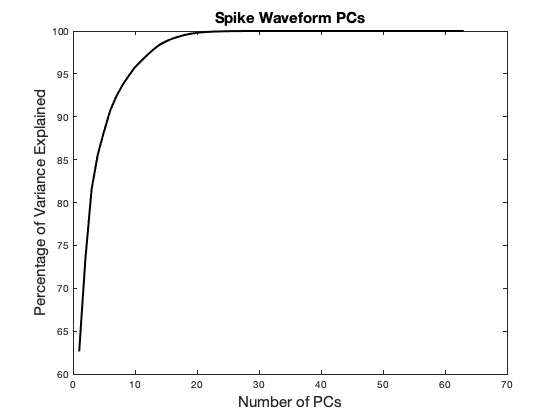
\includegraphics [width=5in]{spatank_hw6_09.png}

	  \item Does it look like there is more than one cluster of spikes? (1 pt)
	\end{enumerate}


   \item Use the same \verb|kmeans| function as you used before to cluster the spikes based on these two (normalized) features (the waveforms represented by the top two PCs). You will use a slight twist, though, in that you will perform $k$-medians (which uses the medians instead of the mean for the cluster centers) by using the \verb|'cityblock'| distance metric (instead of the default \verb|'sqEuclidean'| distance). Make a plot similar to that in 2.2.a but now coloring the two clusters red and green. (3 pts)

\begin{lstlisting}
[labels, C] = kmeans(zscore(score(:, 1:2)), 2, 'Distance', 'cityblock');

figure;
hold on
for i = 1:length(vals)
    if labels(i) == 1
        style = 'r.';
    else
        style = 'g.';
    end
    plot(score(i, 1), score(i, 2), style, 'MarkerSize', 10)
end
hold off
xlabel('1st Principal Component', 'FontSize', 15)
ylabel('2nd Principal Component', 'FontSize', 15)
legend('Cluster 1', 'Cluster 2');
title('Spike Waveform PCs', 'FontSize', 15);
\end{lstlisting}


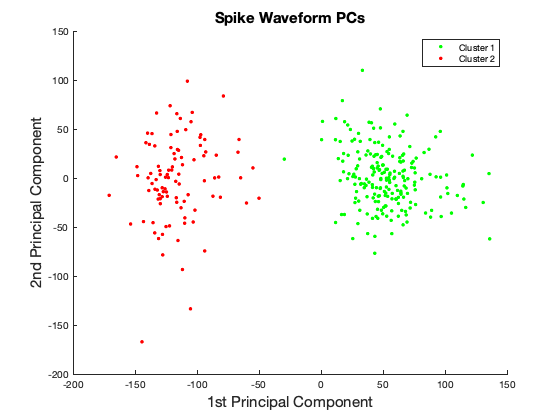
\includegraphics [width=5in]{spatank_hw6_10.png}

  \item Make a plot similar to 2.1 but now coloring the traces red and green according to which cluster they are in. Overlay the mean of the waveforms in each cluster with a thick black line (use the parameter \verb|'LineWidth'| and value \verb|'4'|). (3 pts)

\begin{lstlisting}
figure; cla;
hold on
for i = 1:length(vals)
    if labels(i) == 1
        color = 'r';
    else
        color = 'g';
    end
    curr_spike_start = inds(i);
    all_waveforms(i, :) = ...
        signal(inds(i) - half_window_size:inds(i) + half_window_size);
    plot(pseudo_time, all_waveforms(i, :), 'LineWidth', 0.25, 'Color', color, ...
        'MarkerSize', 10);
end
plot(pseudo_time, mean(all_waveforms(labels == 1, :)), ...
    'LineWidth', 4, 'Color', 'k');
plot(pseudo_time, mean(all_waveforms(labels == 2, :)), ...
    'LineWidth', 4, 'Color', 'k');
hold off
xlabel('Time from Spike (ms)', 'FontSize', 15);
ylabel('Signal ({\mu}V)', 'FontSize', 15);
title('Spike Waveform', 'FontSize', 15);
\end{lstlisting}


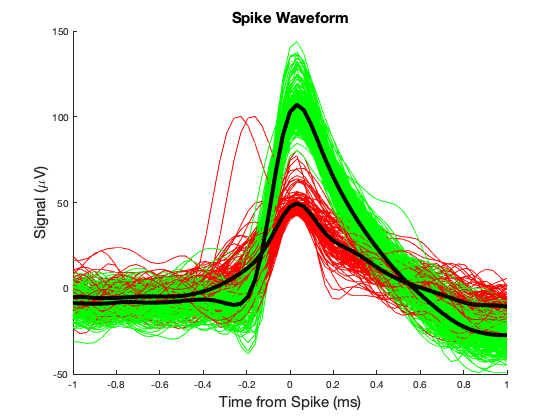
\includegraphics [width=5in]{spatank_hw6_11.png}

  \item What is a disadvantage of using principal component analysis? (1 pts)


  \item What are some dangers of using the clustering techniques in this homework? (List 3) (3 pts)


\end{enumerate}
\end{document}




\end{document}
    
